\documentclass[12pt,a4paper]{article}
\usepackage[utf8]{inputenc}
\usepackage{amsmath}
\usepackage{amsfonts}
\usepackage{amssymb}
\usepackage[brazil]{babel}
\usepackage{indentfirst}
\usepackage{url}
\usepackage{float}
\usepackage{color}
%%%%%%%%%%Codigos para o JAVA%%%%%%%%%%%%%%%%%%%%%%%%%%%%%%%%
\definecolor{pblue}{rgb}{0.13,0.13,1}
\definecolor{pgreen}{rgb}{0,0.5,0}
\definecolor{pred}{rgb}{0.9,0,0}
\definecolor{pgrey}{rgb}{0.46,0.45,0.48}
\usepackage{listings}
\lstset{language=Java,
  showspaces=false,
  showtabs=false,
  breaklines=true,
  showstringspaces=false,
  breakatwhitespace=true,
  commentstyle=\color{pgreen},
  keywordstyle=\color{pblue},
  stringstyle=\color{pred},
  basicstyle=\ttfamily,
  moredelim=[il][\textcolor{pgrey}]{\$\$},
  moredelim=[is][\textcolor{pgrey}]{\%\%}{\%\%}
}
%%%%%%%%%%%%%%%%%%%%%%%%%%%%%%%%Fim codigo JAVA%%%%%%%%%%%%%%
%%%%%%%%%%%Codigo geral%%%%%%%%%%%%%%%%%%%%%%%%%%%%%%%%%%%%%%
\definecolor{mygreen}{rgb}{0,0.6,0}
\definecolor{mygray}{rgb}{0.5,0.5,0.5}
\definecolor{mymauve}{rgb}{0.58,0,0.82}
\lstset{ %
  backgroundcolor=\color{white},   % choose the background color; you must add \usepackage{color} or \usepackage{xcolor}; should come as last argument
  basicstyle=\footnotesize,        % the size of the fonts that are used for the code
  breakatwhitespace=false,         % sets if automatic breaks should only happen at whitespace
  breaklines=true,                 % sets automatic line breaking
  captionpos=b,                    % sets the caption-position to bottom
  commentstyle=\color{mygreen},    % comment style
  deletekeywords={...},            % if you want to delete keywords from the given language
  escapeinside={\%*}{*)},          % if you want to add LaTeX within your code
  extendedchars=true,              % lets you use non-ASCII characters; for 8-bits encodings only, does not work with UTF-8
  frame=single,                    % adds a frame around the code
  keepspaces=true,                 % keeps spaces in text, useful for keeping indentation of code (possibly needs columns=flexible)
  keywordstyle=\color{blue},       % keyword style
  language=Octave,                 % the language of the code
  morekeywords={*,...},            % if you want to add more keywords to the set
  numbers=left,                    % where to put the line-numbers; possible values are (none, left, right)
  numbersep=5pt,                   % how far the line-numbers are from the code
  numberstyle=\tiny\color{mygray}, % the style that is used for the line-numbers
  rulecolor=\color{black},         % if not set, the frame-color may be changed on line-breaks within not-black text (e.g. comments (green here))
  showspaces=false,                % show spaces everywhere adding particular underscores; it overrides 'showstringspaces'
  showstringspaces=false,          % underline spaces within strings only
  showtabs=false,                  % show tabs within strings adding particular underscores
  stepnumber=1,                    % the step between two line-numbers. If it's 1, each line will be numbered
  stringstyle=\color{mymauve},     % string literal style
  tabsize=2,                       % sets default tabsize to 2 spaces
  title=\lstname                   % show the filename of files included with \lstinputlisting; also try caption instead of title
}
%%%%%%%%%%%%%%%%%%%%%%%%%%%%%%%%Fim codigo geral%%%%%%%%%%%%%
\RequirePackage{graphicx}
\title{Vantagens e Desvantagens do Uso de Triggers}
\author{Daniel Moreira Cardoso \and Davi Ildeu de Faria \and Igor Justino Rodrigues \and Luciano de Carvalho Borba \and Warley Rodrigues de Andrade}
 
\usepackage[left=3cm,right=3cm,top=2cm,bottom=2cm]{geometry}
\begin{document}
\begin{titlepage}
\begin{center}
\begin{figure}[htb]
                
                \label{figura:LogoIF}
        
                \centering
                
\includegraphics[width=6cm]{recursos/imagens/logo.png} 
\end{figure}
Instituto Federal Goiano - Campus Ceres\\
Bacharelado em Sistemas de Informação\\
Prof. Me. Ronneesley Moura Teles\\\vspace{0.5cm}
Daniel Moreira Cardoso \\
Davi Ildeu de Faria \\
Igor Justino Rodrigues \\
Luciano de Carvalho Borba \\
Warley Rodrigues de Andrade \\
\vspace{5.0cm}
\textit{\textbf{\Large{Vantagens e Desvantagens do Uso de Triggers}}}\\\vspace{0.5cm}
\vspace{9.5cm}
\end{center}
\end{titlepage}
\tableofcontents
\newpage
\begin{center}
\textbf{\Large{Vantagens e Desvantagens do Uso de Triggers}}\\\vspace{0.5cm}
\end{center}
\section{Introdução}
\subsection{O que é trigger?}

Trigger também conhecida como “Gatilho”  é um objeto de base que é associado com uma tabela e é ativado quando um evento especial acontece, auxiliando uma tabela sempre que é necessário.
A Trigger não é chamada nem é executada, ela é disparada automaticamente como consequência de alterações em tabelas no banco de dados: INSERT, DELETE e UPDATE. Normalmente esse mecanismo é utilizado para manter a integridade dos dados realizando alterações de dados de uma forma sistemática. Um bom exemplo disso é na inserção de dados em uma determinada tabela, usando a forma convencional seria necessário a inserção dos dados de tabela em tabela tornando esse ato um pouco repetitivo e demorado. Já com o uso das triggers a inserção pode ser realizada em várias tabelas ao mesmo tempo agilizando o processo.  Além das Triggers, alguns SGBD possuem outros mecanismos de integridade, como Constraint e Assertion.


\section{Para que serve uma trigger?}
Uma Trigger é dividida em três partes:

\begin{enumerate}


\item Evento: tipo de evento que será executado.
\item Condição: necessidade de executar ou não a ação.
\item Ação: sequência de comandos que serão executadas.
\end{enumerate}

Outra utilização das Triggers está no processo de replicação (cópia) de dados, armazenando os dados de forma redundante para evitar associações frequentes de tabela e a implantação de regras de negócios complexas.

\section{Portabilidade de Sistema Gerenciador de Banco de Dados (SGBD)}
”Ao adotar Trigger resultará na quase impossibilidade de migração de banco de dados.” 
Frase destacada no \url{forumrm.com}
 
Um dos principais e maiores problemas do uso das triggers é realmente a portabilidade, em diversos fóruns de TI existe quase uma unanimidade nas opiniões em relação a esse assunto.
As triggers são criadas exclusivamente para o banco de dados utilizado, caso posteriormente seja necessário a troca do SGBD as triggers terão que ser recriadas adaptando-as para o  SGBD escolhido, causando assim uma pequena dor de cabeça.
Diversos programadores que utilizam trigger por real necessidade apontam esse problema como principal motivo de descontentamento em relação ao uso das triggers. 

\section{Exemplos}
\subsection{O que utilizamos?}
Para realizar comparações fizemos uso do PostgreSQL, um excelente SGBD que além de opensource, possui uma interface bastante amigável com o pgAdmin 4.
\begin{figure}[h]
\centering
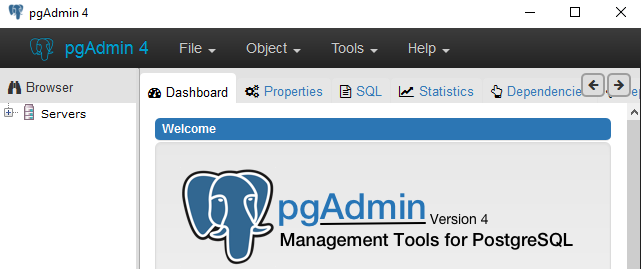
\includegraphics[width=15cm]{recursos/imagens/postgre.png}
\label{1}
\caption{Postgre e pgAdmin 4. Fonte:https://i.stack.imgur.com/JLp68.png; Acesso em 08/11/2017}
\end{figure}

E também utilizamos o Mysql, com o Mysq Workbench, que acreditamos que todos conheçam.
\begin{figure}[h]
\centering

\includegraphics[width=15cm]{recursos/imagens/mysql.jpg}
\label{2}
\caption{Mysql e Mysql Workbench. Fonte:https://i.ytimg.com/vi/-GnKwwc4KSA/maxresdefault.jpg; Acesso em 08/11/2017}
\end{figure}

\subsection{PostgreSQL}

\lstinputlisting{recursos/sql/POSTGRE.sql}

\subsection{Mysql}

\lstinputlisting{recursos/sql/MYSQL.sql}

\section{Vantagens e Desvantagens}
\subsection{Vantagens}
\begin{itemize}
\item Uma forma a mais para garantir a integridade dos dados.
\item São capazes de detectar erros na lógica de negócios na camada do banco de dados.
\item Uma forma para executar tarefas no banco.
\item Muito utilizado para auditar modificações(deletes ou updates) no banco.
\end{itemize}

\subsection{Desvantagens}
\begin{itemize}
\item Validador de apenas uma parte das informações.
\item Por ele ser executado na camada do banco de dados, fica complicado ao usuário saber o que está
ocorrendo no BD.
\item Pode causar uma demora a mais no processamento no servidor do banco.
\item As triggers são feitas especialmente para determinado SGBD, por isso uma mudança deste para outro SGBD obrigaria a adaptar todas as triggers.
\end{itemize}

\section{Conclusão}

Pela observação dos aspectos analisados concluímos que para utilização das trigger somente se existir real necessidade de uso, caso contrário é dispensável.
Já que mesmo apresentando muitas vantagens deixa a desejar em relação a portabilidade, a portabilidade tem como subcaracterísticas: adaptabilidade, capacidade de instalação, conformidade e capacidade de substituição.  




\end{document}
%Modelo de código para inserir figura
%\begin{figure}[h]
%\centering
%
\includegraphics[width=15cm]{logo.png}
%\label{4}
%\caption{Fonte:http://...; Acesso em 06/11/2017}
%\end{figure}